\documentclass[a4paper]{jpconf}
\usepackage{graphicx}
\usepackage{multirow}

\bibliographystyle{LaTexTemplates/BibTeX/iopart-num/iopart-num}


\begin{document}
\title{First measurements of muon production rate using a novel pion capture system at MuSIC}

\author{S~Cook$^1$, R~D'Arcy$^1$, M~Fukuda$^2$, K~Hatanaka$^2$, Y~Hino$^3$, Y~Kuno$^3$, M~Lancaster$^1$, Y~Mori$^4$, TH~Nam$^3$, T~Ogitsu$^5$, H~Sakamoto$^3$, A~Sato$^3$, NM~Truong$^3$, A~Yamamoto$^5$, M~Yoshida$^5$ and M~Wing$^1$}

\address{$^1$Department of Physics and Astronomy, University College London, Gower Street, London WC1E~6BT, UK}
\address{$^2$Research Centre for Nuclear Physics, 10-1 Mihogaoka, Ibaraki, Osaka~567-0047, Japan}
\address{$^3$Department of Physics, Graduate School of Science, Osaka University, 1-1 Machikane, Toyonaka, Osaka 590-0043 Japan}
\address{$^4$Kyoto Research Reactor Institute, 2 Asashiro-Nishi, Kumatori-cho, Sennangu, Osaka 590-0494, Japan}
\address{$^5$High Energy Accelerator Research Organisation, KEK, 1-1 Oho, Tsukuba, Ibaragi 305-0801, Japan}

\ead{scook@hep.ucl.ac.uk}

\begin{abstract}
The MuSIC (Muon Science Innovative Channel) beam line at RCNP (Research Centre for Nuclear Physics), Osaka will be the most intense source of muons in the world. A proton beam is incident on a target and, by using a novel capture solenoid, guides the produced pions into the beam line where they subsequently decay to muons. This increased muon flux will allow more precise measurements of cLFV (charged Lepton Flavour Violation) as well as making muon beams more economically feasible. Currently the first 36$^{\circ}$ of solenoid beam pipe have been completed and installed for testing with low proton current of 1~nA. Measurements of the total particle flux and the muon life time were made. The measurements were taken using thin plastic scintillators coupled to MPPCs (Multi-Pixel Photon Counter) that surrounded a magnesium or copper stopping target. The scintillators were used to record which particles stopped and their subsequent decay times giving a muon yield of $8.5\times 10^5 \rm{~muons} \rm{~W}^{-1}_{\rm{proton~beam}}$ or $3\times 10^8 \rm{~muons} \rm{~s}^{-1}$ when using the RCNP's full power (400~W).
\\
\\ 
% Contribution to: NUFACT 11, XIIIth International Workshop on Neutrino Factories, Super beams and Beta beams, 1-6 August 2011, CERN and University of Geneva (Submitted to IOP conference series).

\end{abstract}    

\section{Introduction}
The Muon Science Innovative Channel (MuSIC) aims to generate the most intense muon beam in the world. More importantly it aims to have the highest proton to muon yield in the world. Muons are increasingly becoming of interest for those wanting to probe the energy and precision frontiers; MuSIC hopes to provide the technology to make it possible to pursue  these aims.

Creating a high intensity muon beam will open up many areas of research. Planned programs include: precision measurements of $\mu \rightarrow eee$; research and development into using FFAGs as muon storage rings; nuclear muon capture; and material science use of the muon beam such as muon spin rotation. Further in the future, high intensity muon beams can be used to drive neutrino factories and muon colliders. 

\begin{figure}[htbp]
    \centering
        % 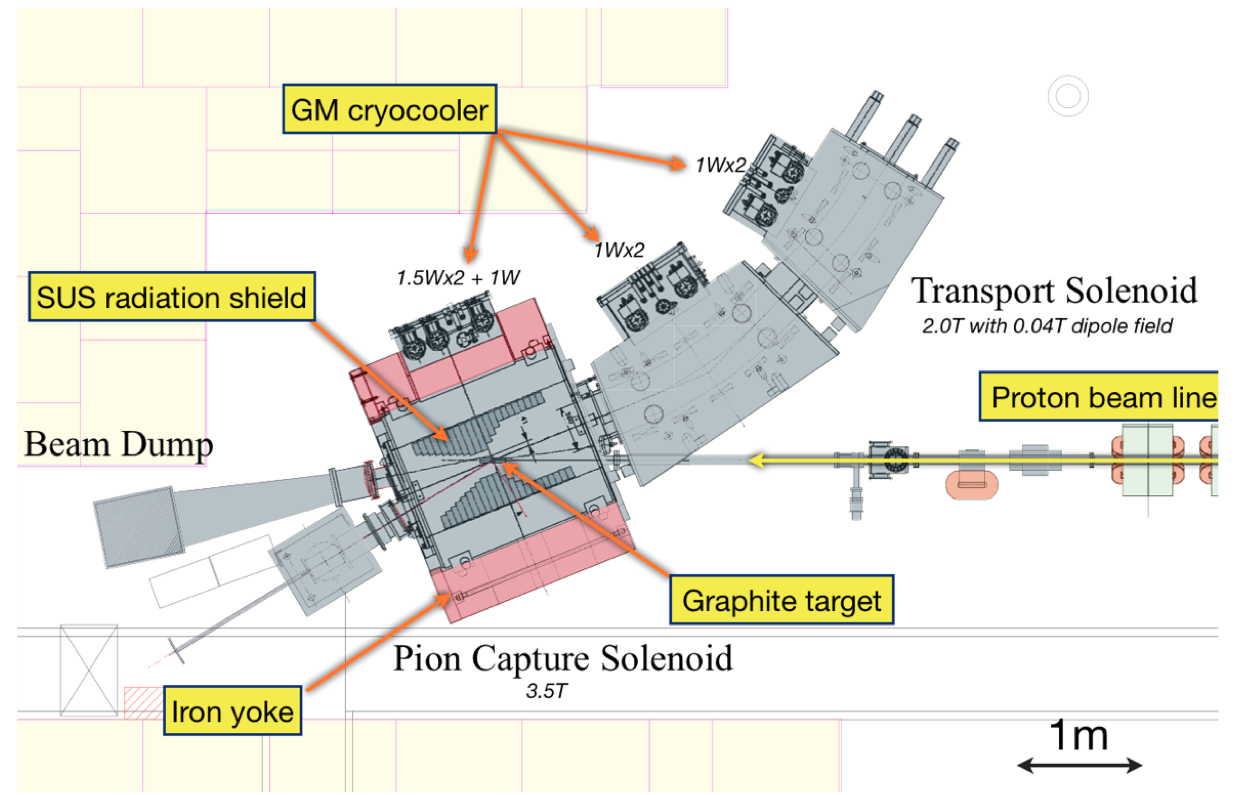
\includegraphics[height=6cm]{images/MuSIC_current_schematic.png}
        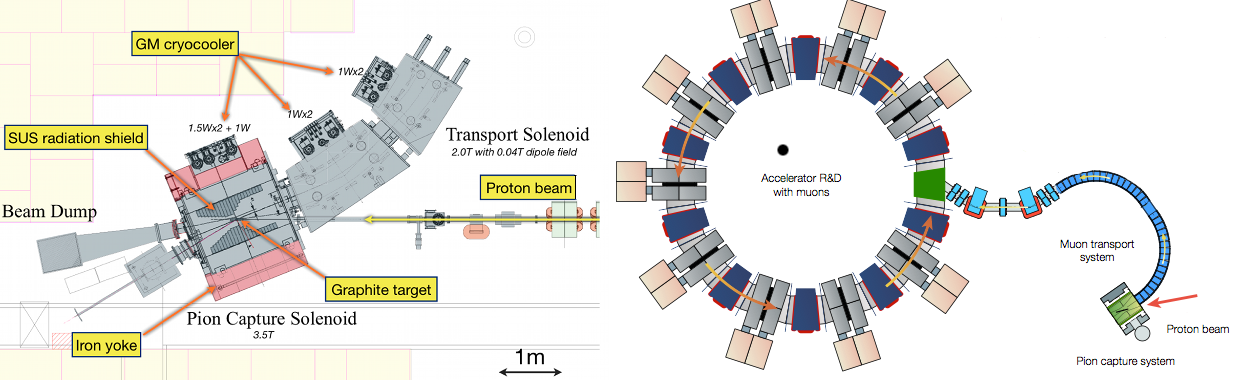
\includegraphics[width=16cm]{images/MuSIC_current_schematic2.png}
    \caption{Left, a schematic of the current status of the MuSIC pion production system. Right, the proposed, fully completed, facility.}
    \label{fig:MuSIC_schematic}
\end{figure}
\section{Overview}
MuSIC is a muon beam line being built at the Research Centre for Nuclear Physics (RCNP) in Osaka, Japan. In addition to using the majority of the proton beam in pion production it also employs a novel pion capture solenoid to vastly increase its proton to muon efficiency. 

The pion capture solenoid provides nearly 2$\pi$~Sr acceptance in the production region. This captures backwards travelling pions using a 3.5~T superconducting magnet that completely surrounds the production target. The target is a 20~cm long graphite cylinder with a radius of 2~cm.

Stainless steel shielding is used to protect the superconducting solenoids from excessive heating. Cooling for the solenoid at 4~K is provided by 3 GM cryocoolers (two with a power of 1.5~W each and one of 1~W). The entire apparatus is enclosed in an iron yoke.  

MuSIC produces muons from the decay of pions; to allow time for this to occur there is a transport solenoid after the capture solenoid, this also provides momentum selection. The transport solenoid has a 3~m diameter and extends for 180$^{\circ}$. It has a static 2~T magnetic field as well as an additional 0.04~T magnetic field that can be used for fine adjustments and charge selection.

The proton beam is supplied by the RCNP cyclotron, it is a 400~W proton beam with maximum current of 1~$\mu$A (with a planned upgrade to 5~$\mu$A) and energy of 392~MeV. It is a continuous proton beam.

Commissioning of MuSIC began in 2009 and consisted of the installation of the pion capture solenoid and the first 36$^{\circ}$ of the transport solenoid. There have been three successful runs, the most recent of which was in July~2011 when the muon component of the beam was measured. The initial runs have been performed using a lower, 1~nA, current pending measurements of the neutron flux which will allow use of the full 1~$\mu$A current.



\section{Measurement of muon flux}
\subsection{Measurement of the muon lifetime}
\begin{figure}[htbp]
    \centering
        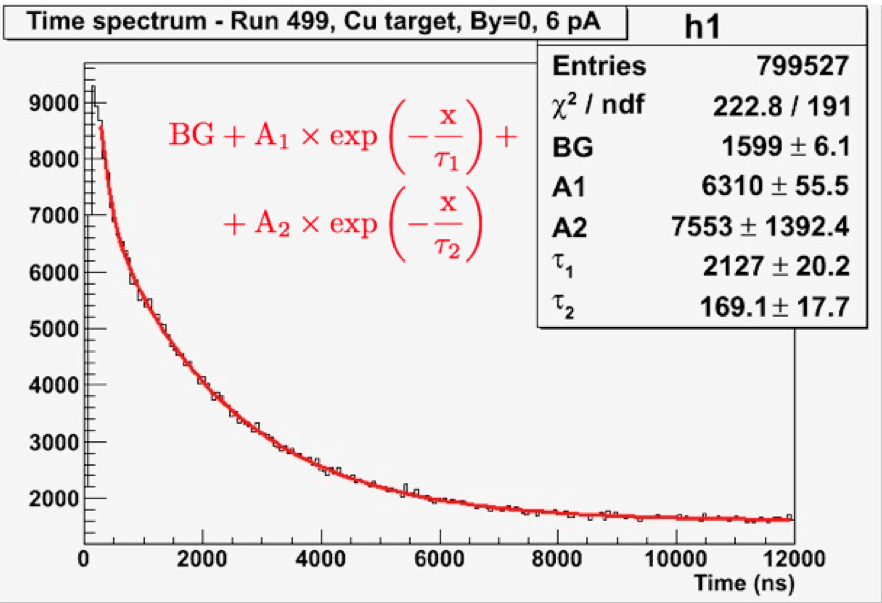
\includegraphics[height=6cm]{images/muon_decay.png}
\caption{Decay time for stopped muons. Fitted with two exponentials, corresponding to the copper stopping time and the combination of free muon decay times with muons stopping in the scintillator (see table~\ref{tab:muon_halflifes}).}
    \label{fig:muon_decay}
\end{figure}

\begin{table}
    \begin{center}  
	\caption{Muonic decay times. The measured values for plastic scintillator and a free muon are the same as we did not have sufficient data to resolve these two components.}
        \lineup
    \begin{tabular}{l l l l l l}
        \br
        Material               & Measured (ns)  & Expected (ns)           & Ref \cr
        \mr                                                           
        Carbon (scintillator)  & \multirow{2}{*}{2127 $\pm$ 20} &  2026.3\0\0  $\pm$ 1.5   & \cite{Suzuki1987muonCapture} \cr
        Free Muon              &                                &  2197.034    $\pm$ 0.021 & \cite{Pdg2010}               \cr
        Copper                 & \0169 $\pm$ 17                 & \0164.0\0\0 $\pm$ 1.6   & \cite{Suzuki1987muonCapture} \cr
        \br
    \end{tabular}
    \end{center}
    % \caption{Muonic decay times. The measured value for plastic scintillator and a free muon is the same as we did not have the data needed to resolve these two components.}
    \label{tab:muon_halflifes}
\end{table}
In order to establish both the presence of muons in the beam and their flux the muon lifetime was measured. The experimental set up consisted of two plastic scintillators (both $400\times 50\times 3.5$~mm$^3$) on either side of a copper stopping target ($370\times 80\times 6$~mm$^3$). This arrangement was held in place using an aluminium surround positioned at the end of the beam pipe. 

To measure the lifetime a simple trigger system was devised to detect stopped muons and then measure the time taken for the decay electron to be emitted. A gate of 20~$\mu$s was used to look for the decay electron. The logic for detection of a muon was a hit in the front scintillator but not the rear whilst an electron was taken as a single hit in either the front or the rear scintillator. 

A multi-hit TDC was used to time every hit that triggered only one of the scintillators after the initial muon. Readout from the scintillators was done using MPPCs which have an output signal proportional to the number of photons that strike their surface. MPPCs were used instead of traditional PMTs as they work well in strong magnetic fields and can be directly mounted to the scintillator without light guides, which reduces the cost and complexity of the system. 

The beam supplied during the measurement was a 6~pA proton beam at 392~MeV. This exceeds the pion production threshold.

A preliminary analysis has been carried out in which two exponential curves and a constant background have been fitted to the data (figure~\ref{fig:muon_decay}). The two exponentials accounted for the decay of negative muons in Cu; and a combined term for decay of free muons or muons captured in the plastic scintillator (carbon capture). The approximation of the capture of muons in carbon for capture in plastic is discussed in \cite{Suzuki1987muonCapture}. The measurement of the muon in copper was 169$\pm$17~ns whilst the measured combined value for a free muon and muon in carbon is 2127$\pm$20~ns given in table~\ref{tab:muon_halflifes}. As muon capture only occurs for negative muons we can use the ratio of the deviations from the predicted values as a measure of the ratio of positive to negative muons ($R$) using the equation:
\begin{eqnarray}
    R &= \frac{\tau_{\rm{measured}} - \tau_{\rm{C}}}{\tau_{\rm{free}} - \tau_{\rm{C}} } = \frac{2127 - 2026}{2197-2026} \approx 0.6  \label{equ:ratio_pos_neg}
\end{eqnarray}
Where $\tau_{\rm{measured}}$ our measurement of the muon lifetime and $\tau_{\rm{C}}$ and $\tau_{\rm{free}}$ are the lifetimes given in \cite{Suzuki1987muonCapture} and \cite{Pdg2010} respectively. Finally using the rate at which the system was triggered with stopped muons a measure of the muon rate gives a beam current of 2000~muons~s$^{-1}$ this implies a rate of 3$\times 10^8$ muon s$^{-1}$ should be achievable when using the full proton beam current of 1~$\mu$A. 

\begin{figure}[htbp]
    \centering
        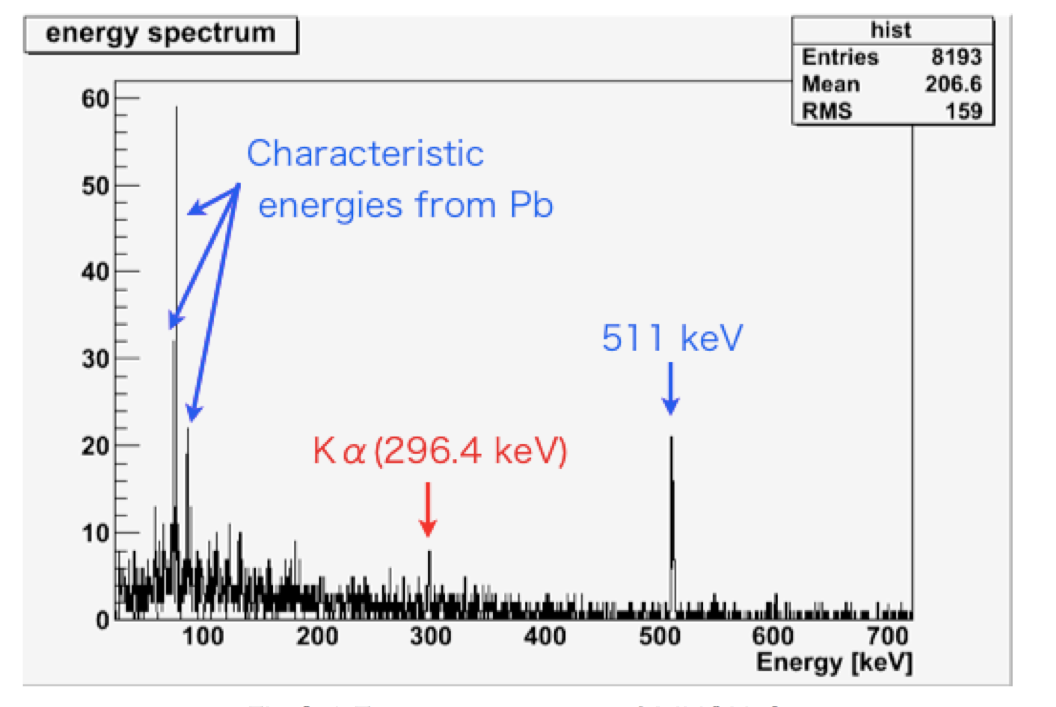
\includegraphics[height=7.5cm]{images/muonic_xray_spectrum.png}
    \caption{Energy spectrum of X-rays detected using the Ge detector. The three low energy peaks are due to emissions from the surrounding lead, the peak 511~KeV is due to electron-positron annihilation, the K$\alpha$ peak is produced by muonic magnesium; 26 entries were counted at the K$\alpha$ peak, this corresponds to a muon flux of 10$^8$ muons s$^{-1}$ given a 1~$\mu$A proton beam.}
    \label{fig:muonic_xray_spectrum}
\end{figure}
\subsection{Measurement of muon X-rays}
As well as measuring the muon lifetime in copper the emission of X-rays from muonic magnesium was also measured. This was done using a Ge detector.

The detector was set slightly back from the end of the beam pipe and shielded from stray radiation using lead, paraffin and cadmium. Using the scintillators to reject non-stopping muons an energy spectrum of the detected X-rays was constructed and the K$\alpha$ muonic peak identified (figure~\ref{fig:muonic_xray_spectrum}). Preliminary estimates accounting for acceptance of the Ge detector imply that the number of muonic X-rays seen correspond to a flux of $10^8$ muons s$^{-1}$ when using a 1$\mu$A proton beam.

\section{The prospects}
At time of writing a fourth beam time is being planned to measure the background neutron flux in order to establish whether further shielding is required. Assuming a successful run then beam time is scheduled for early 2012 in order to begin using higher beam currents with the ultimate aim of measuring the highest intensity muon beam in the world. Beyond that it is hoped that the commissioning of the complete facility can be completed in the next 4 years.
\section*{References}
\bibliography{nufact}
\end{document}
















